\documentclass[10pt]{beamer}

\usepackage{polyglossia}
\usepackage{adjustbox}
\usepackage{csquotes}
\usepackage{datetime}
\usepackage{fontspec}
\usepackage{microtype}
\usepackage{color}
\usepackage{url}
\usepackage{hyperref}
\usepackage{amsfonts}
\usepackage{amsmath}
\usepackage{amsthm}
\usepackage{subcaption}
\usepackage[backend=biber,style=iso-authoryear,sortlocale=en_US,autolang=other,bibencoding=UTF8]{biblatex}
\usepackage{booktabs}
\usepackage{graphics}
\usepackage{pifont}
\usepackage{ulem}
\usepackage{tikz}

\addbibresource{zotero.bib}

\setdefaultlanguage{english}
\setmainfont{TeX Gyre Termes}
\usetheme{Boadilla}
\usecolortheme{crane}
\setbeamertemplate{title page}[default][rounded=true,shadow=false]
\setbeamertemplate{section in toc}[ball unnumbered]
\setbeamertemplate{bibliography item}{}

\hypersetup{%
	pdfencoding=auto,
	unicode=true,
	citecolor=green,
	filecolor=blue,
	linkcolor=red,
	urlcolor=blue
}

\makeatletter
\newcommand*{\currentSection}{\@currentlabelname}
\makeatother

%\newcommand{\mathmat}{\ensuremath{\mathbf}}
\newcommand{\vdeg}{\mathrm{d}} % degree of node or edge
\newcommand{\edeg}{\delta} % degree of node or edge

\title[PhD proposal]
{%
	Representation learning for structured data
}

\newdate{presentation}{29}{11}{2024}
\date[November 2024]{FJFI ČVUT, \displaydate{presentation}}

\author[Marek Dědič]
{%
	Marek~Dědič\inst{1}, \\ \vspace{8pt}
	\footnotesize{Superviser: prof.~RNDr.~Ing.~Martin~Holeňa,~CSc.}\inst{2}, \\
	Specialist: Mgr.~Lukáš~Bajer,~Ph.D.\inst{3}
}

\institute[FJFI ČVUT]
{%
	\inst{1} Faculty of Nuclear Sciences and Physical Engineering, Czech Technical University in Prague \and
	\inst{2} Institute of Computer Science, Czech Academy of Sciences \and
	\inst{3} Cisco Systems, Inc.
}

% Title card
\AtBeginSection[]{%
	\begin{frame}
		\vfill
		\centering
		\begin{beamercolorbox}[sep = 8pt,center,shadow = true,rounded = true]{title}
			\usebeamerfont{title}\insertsectionhead\par%
		\end{beamercolorbox}
		\vfill
	\end{frame}
}

%\AtBeginSection[]{%
	%\begin{frame}{\currentSection}
		%\tableofcontents[currentsection]
	%\end{frame}
%}

\begin{document}

\begin{frame}
	\titlepage
\end{frame}

\begin{frame}{Motivation}
	\begin{itemize}
	\item Graphs are a natural way of abstracting many mathematical and real-world problems
	\item Use in chemistry, software engineering, image recognition, medicine, particle physics, network security, fake-news detection, autonomous vehicles etc.
	\end{itemize}

	\centering
	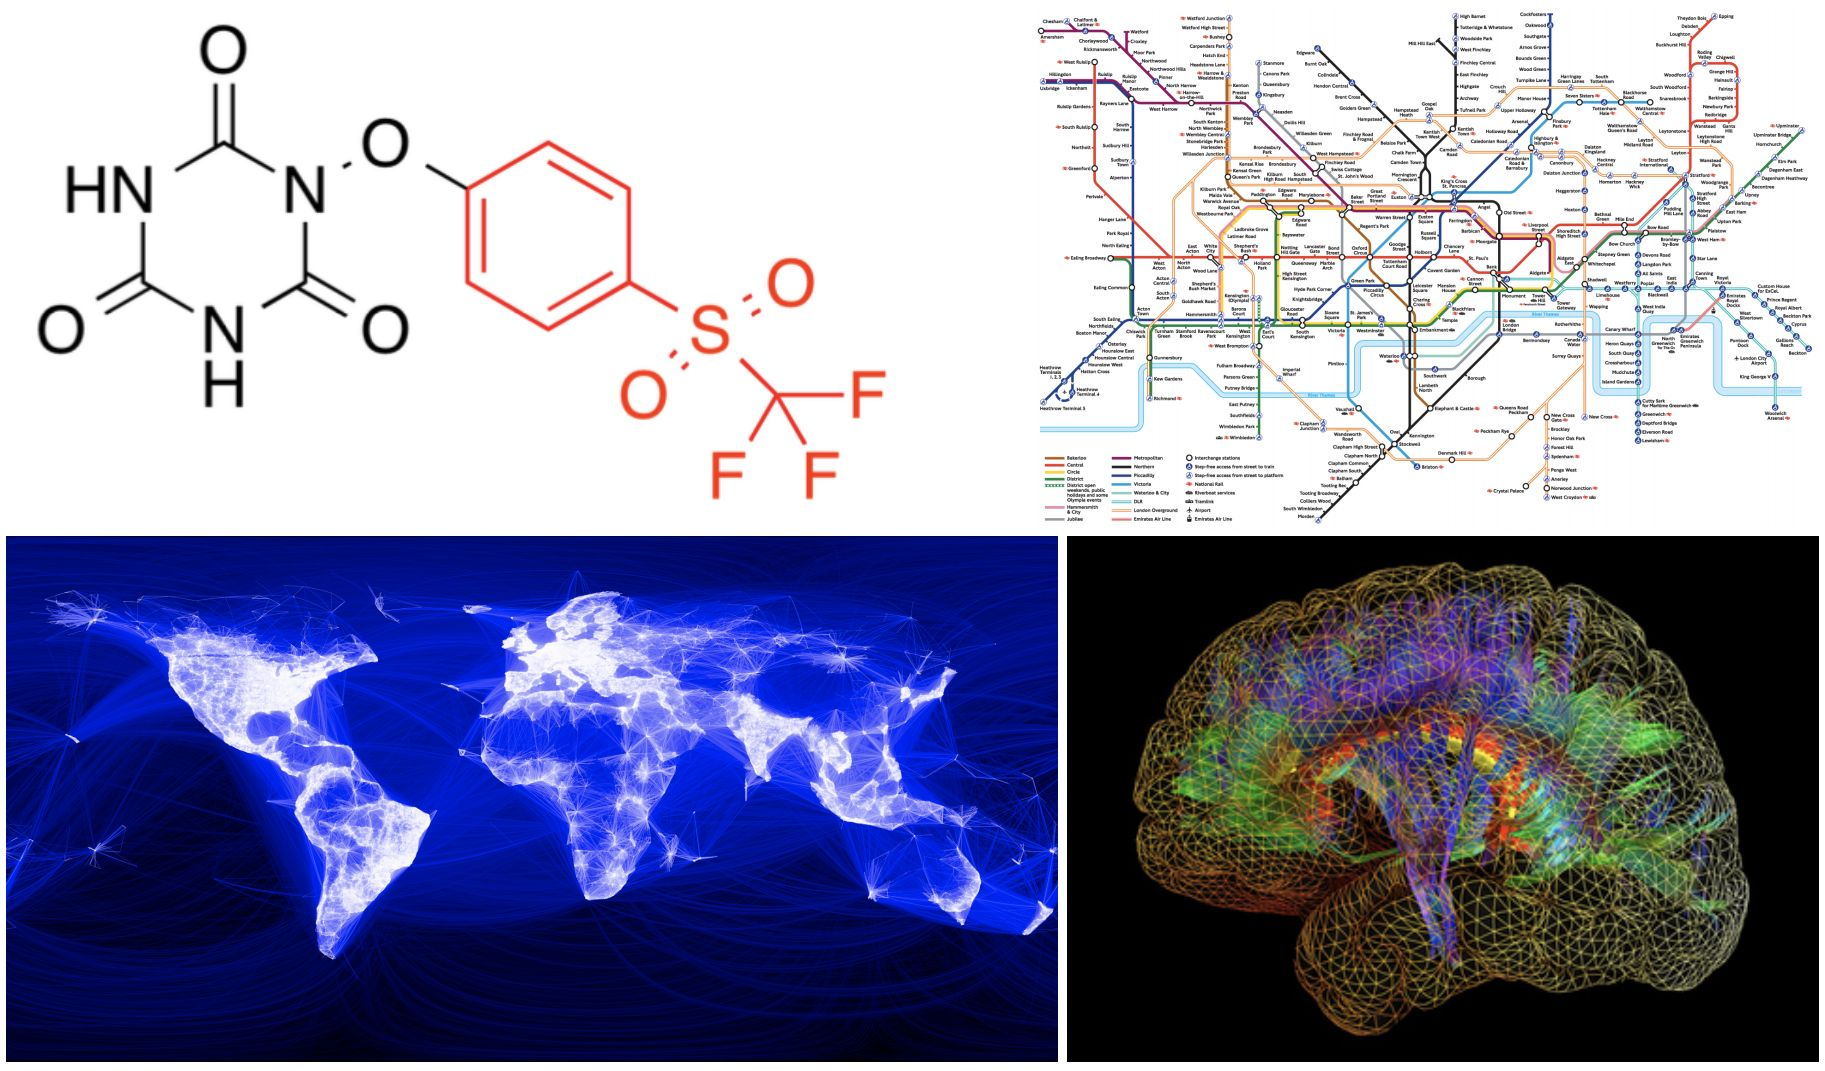
\includegraphics[width=0.7\pagewidth]{images/graphs.png}\footcite{velickovic_opening_2020}
\end{frame}

\begin{frame}{Outline}
	\begin{itemize}
		\item Contributions
		\begin{itemize}
			\item The graph performance-complexity trade-off
			\item A HARP-based approach to solving it
			\item A direct approach to solving it
			\item The effect of graph properties on GNN performance
		\end{itemize}
		\item Intended research directions
		\begin{itemize}
			\item Applications in cybersecurity
			\item Explainable graph models
			\item Hyper-parameter optimisation for GNNs
		\end{itemize}
	\end{itemize}
\end{frame}

\section{Contributions}

\begin{frame}{The performance-complexity trade-off\footcite{prochazka_scalable_2022, dedic_balancing_2023, dedic_balancing_2024}}
	\begin{itemize}
		\item<1|only@1> Sequence of graphs \( G_0, G_1, G_2, \dots, G_L \) where \( G_0 = G \)
		\item<1|only@1> Model \( M \), a performance metric, a complexity metric
		\item<1|only@1> The sequence draws a curve in the performance-complexity space
		\item<2|only@2> Given maximum available complexity $C_m$, we select such a graph that the complexity of the graph is smaller than $C_m$ and achieve performance $P_3$ -- blue arrows.
		\item<2|only@2> Given minimal required performance $P_m$, we select such a graph that $|\mathcal{P}_i|\ge P_m$ with complexity $C_2$ -- green arrows.
	\end{itemize}

	\vfill

	\centering
	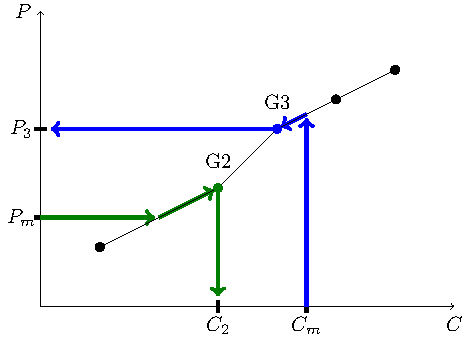
\includegraphics[width=0.6\linewidth]{images/performance-complexity-schema/performance-complexity-schema.pdf}
\end{frame}

\begin{frame}{A HARP-based method for performance-complexity balancing\footcite{dedic_balancing_2024}}
	\begin{itemize}
		\item HARP -- a method for pretraining on simplified graphs
		\item Embedding trained first on the coarser graph
	\end{itemize}

	\vfill

	\centering
	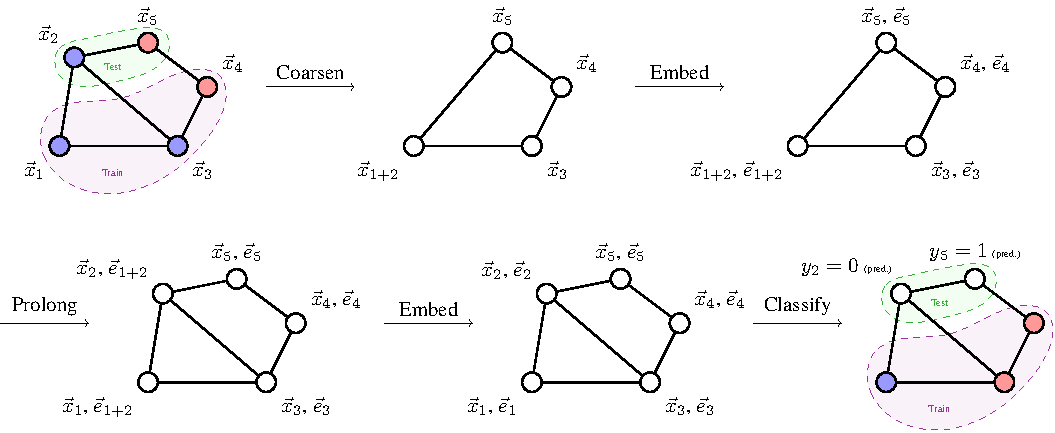
\includegraphics[width=0.9\linewidth]{images/harp-overview/harp-overview.pdf}
\end{frame}

\begin{frame}{A HARP-based method for performance-complexity balancing}
	\begin{itemize}
		\item Sequence of graphs \( G_0, G_1, \dots, G_L \) generated by repeated application of HARP
		\item Embeddings \( \Phi_{G_L}, \dots, \Phi_{G_1}, \Phi_{G_0} \) obtained in reverse
	\end{itemize}

	\vfill

	\centering
	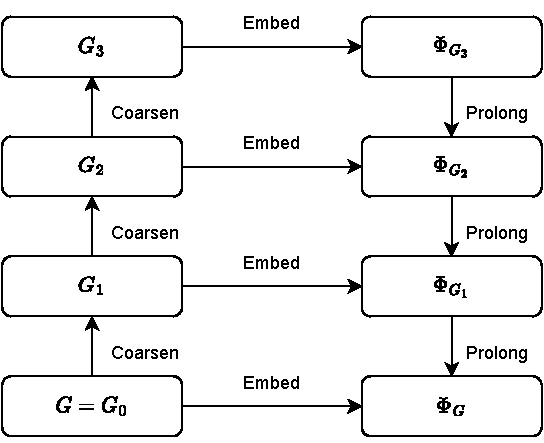
\includegraphics[width=0.5\linewidth]{images/deep-harp/deep-harp.pdf}
\end{frame}

\begin{frame}{A HARP-based method for performance-complexity balancing}
	\begin{itemize}
		\item Main contribution: An adaptive way of embedding prolongation.
	\end{itemize}

	\vfill

	\centering
	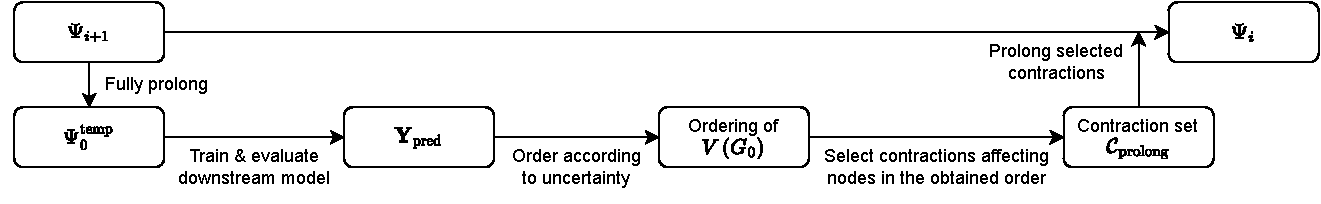
\includegraphics[width=\linewidth]{images/adaptive-prolongation/adaptive-prolongation.pdf}
\end{frame}

\begin{frame}{A HARP-based method for performance-complexity balancing}
	\begin{itemize}
		\item Headline result: At 60\% complexity, the models have over a 99\% probability of being within 10 percentage points of performance on the full graph and at 80\% complexity, they have over 99\% probability of being withing 5 percentage points of performance.
	\end{itemize}

	\vfill

	\centering
	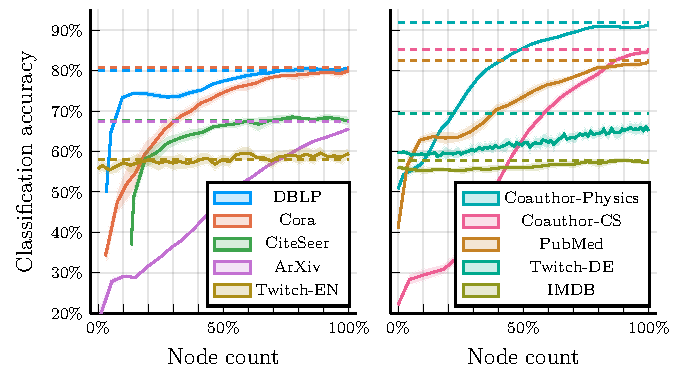
\includegraphics[width=0.7\linewidth]{images/adaptive-coarsening/adaptive-coarsening.pdf}
\end{frame}

\begin{frame}{A direct approach to graph coarsening\footcite{prochazka_scalable_2022}}
	\begin{itemize}
		\item Alternative, direct approach to coarsening
		\item Orders edges based on the similarity of their predictive posterior distribution under an auxiliary model
		\item Edge ordering defines the sequence \( G_0, G_1, \dots, G_L \)
	\end{itemize}

	\vfill

	\centering
	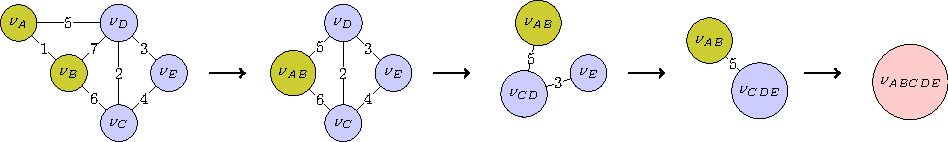
\includegraphics[width=0.9\linewidth]{images/edge-contraction-sequence/edge-contraction-sequence.pdf}
\end{frame}

\begin{frame}{A direct approach to graph coarsening}
	\begin{itemize}
		\item Simpler, less powerful
	\end{itemize}

	\vspace{-25pt}

	\centering
	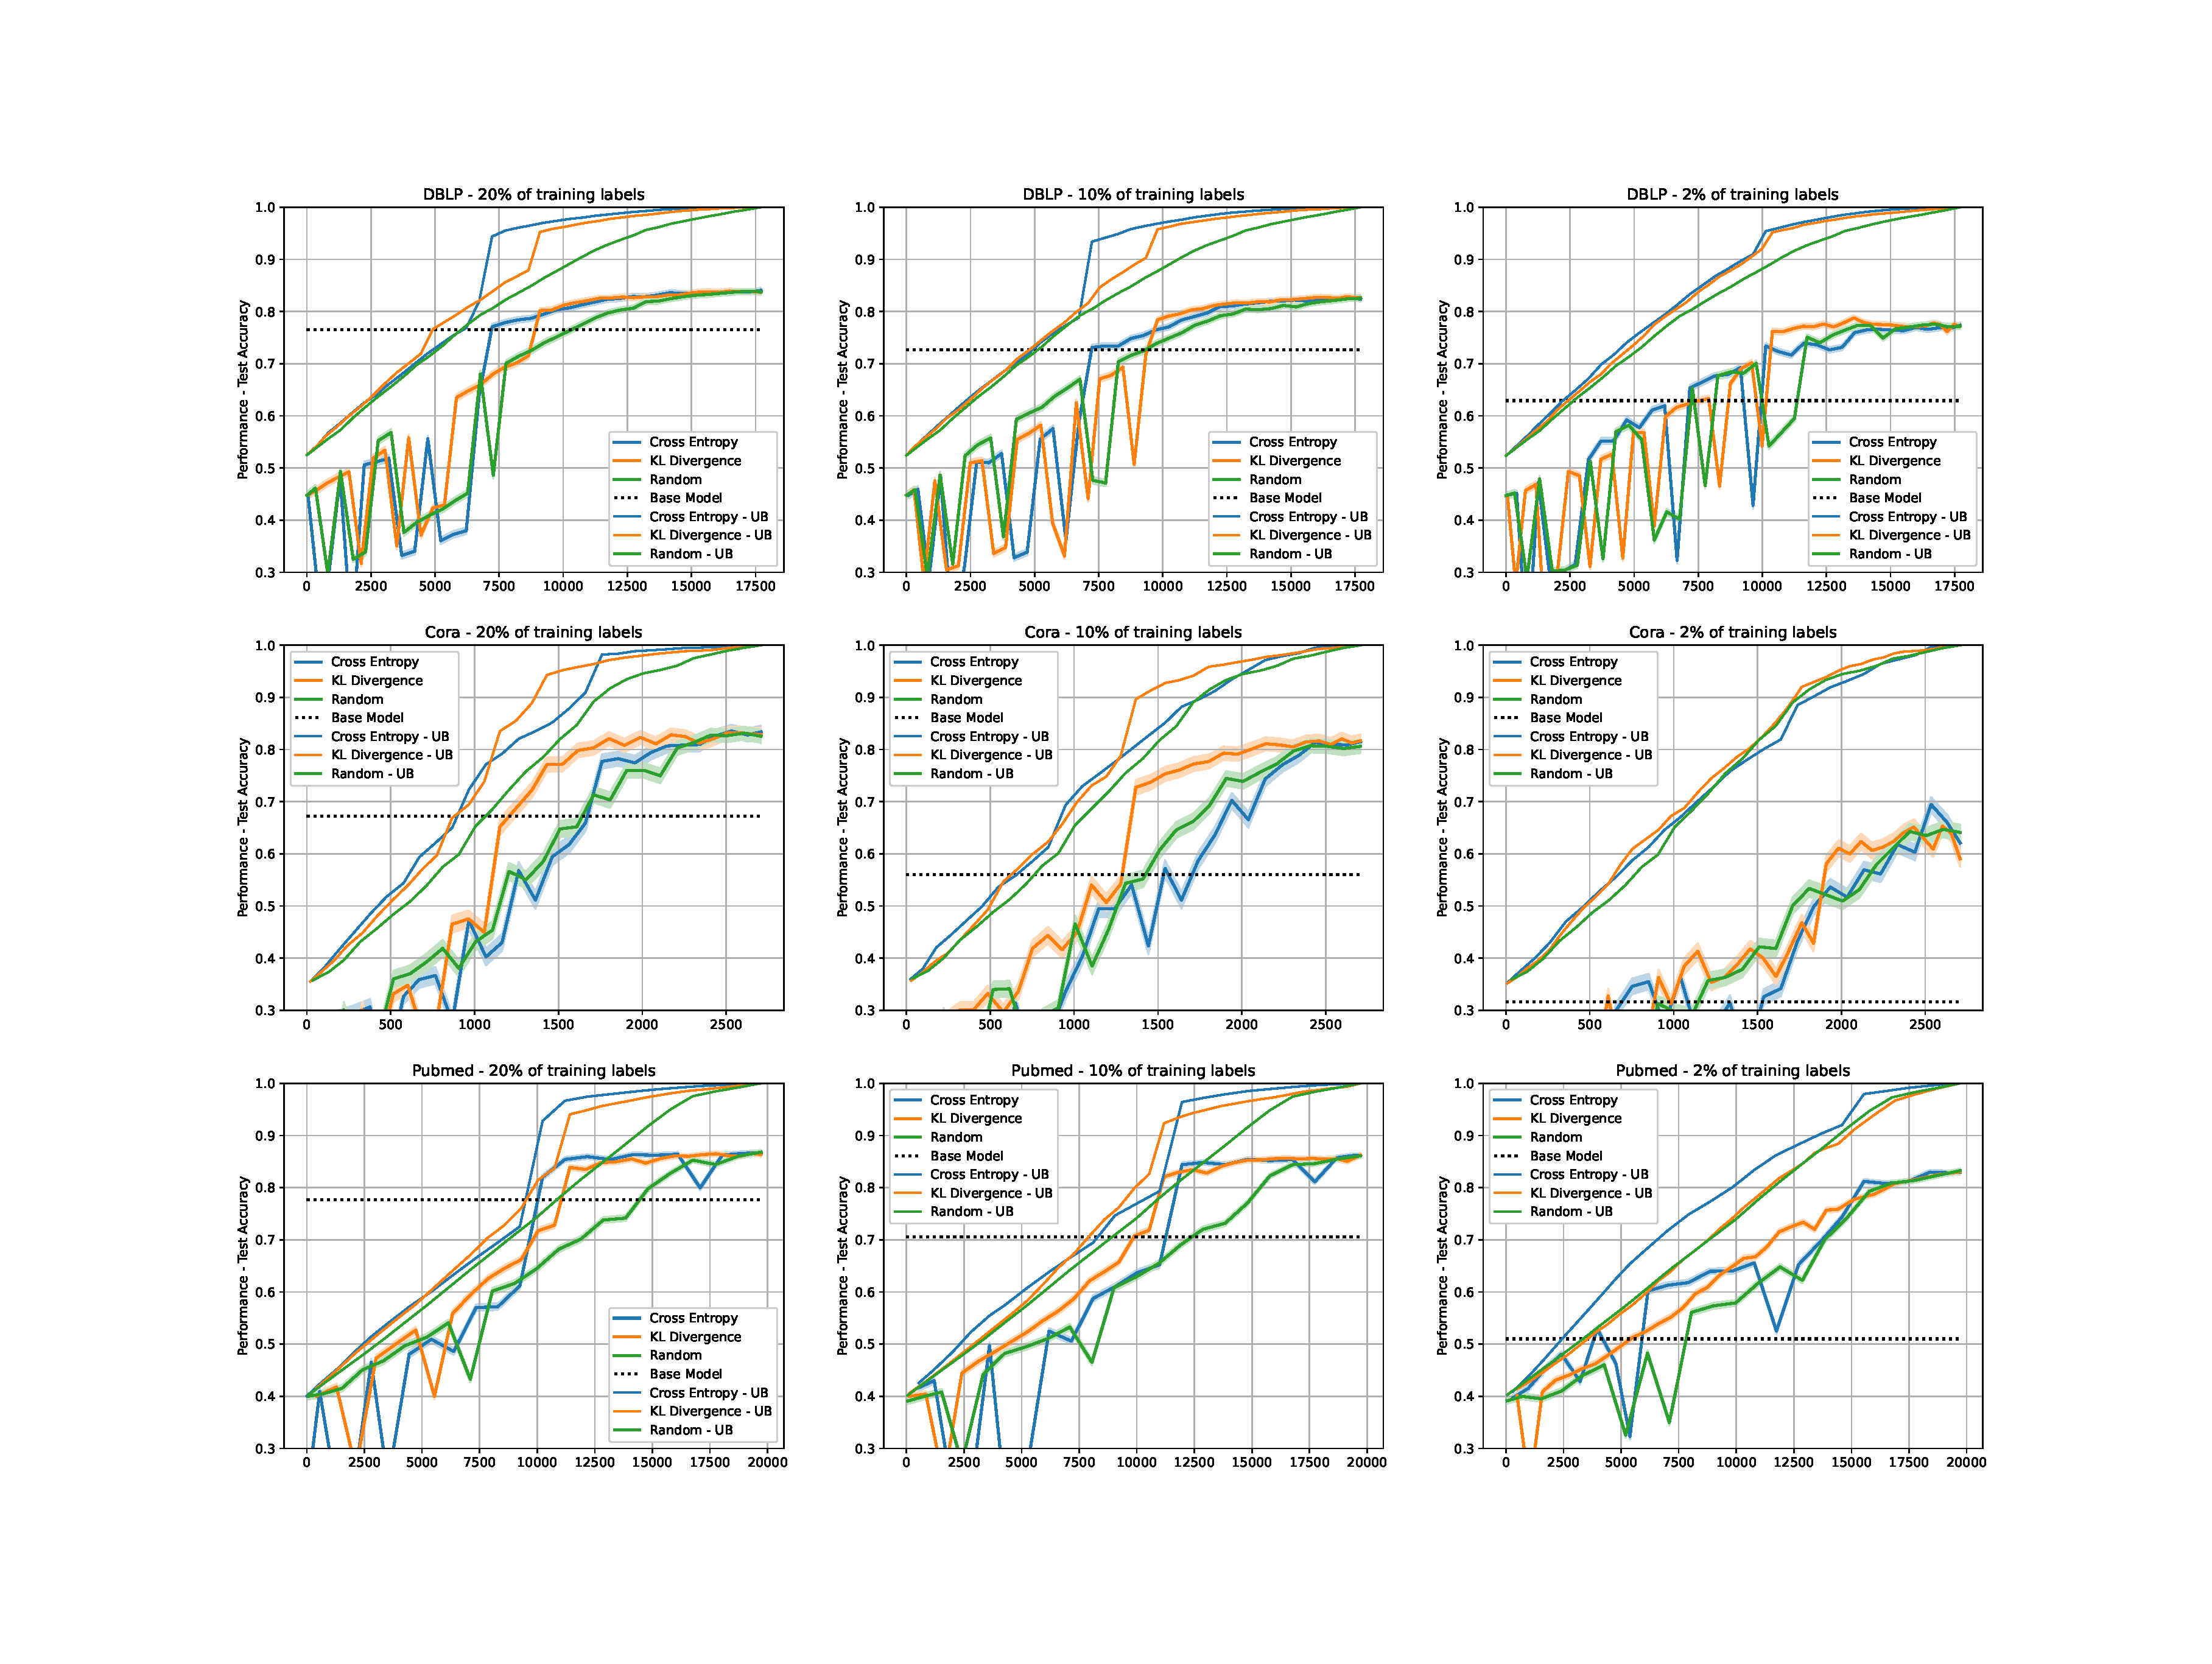
\includegraphics[width=\linewidth]{images/direct-graph-coarsening-results.eps}
\end{frame}

\begin{frame}{The effect of graph properties on downstream task performance\footcite{prochazka_which_2023}}
	\begin{itemize}
		\item How data are transformed into a graph may affect the performance of the downstream task in a profound way.
		\item Step 1: Measuring and predicting the suitability of a given graph representation to a given downstream task.
		\item Measured 17 different graph properties on 7 standard graphs -- 139 data points
		\item Trained a GraphSAGE model and evaluated 5 performance metrics
		\item Using a meta-model, we measured the importance of the properties
	\end{itemize}
\end{frame}

\begin{frame}{The effect of graph properties on downstream task performance}
	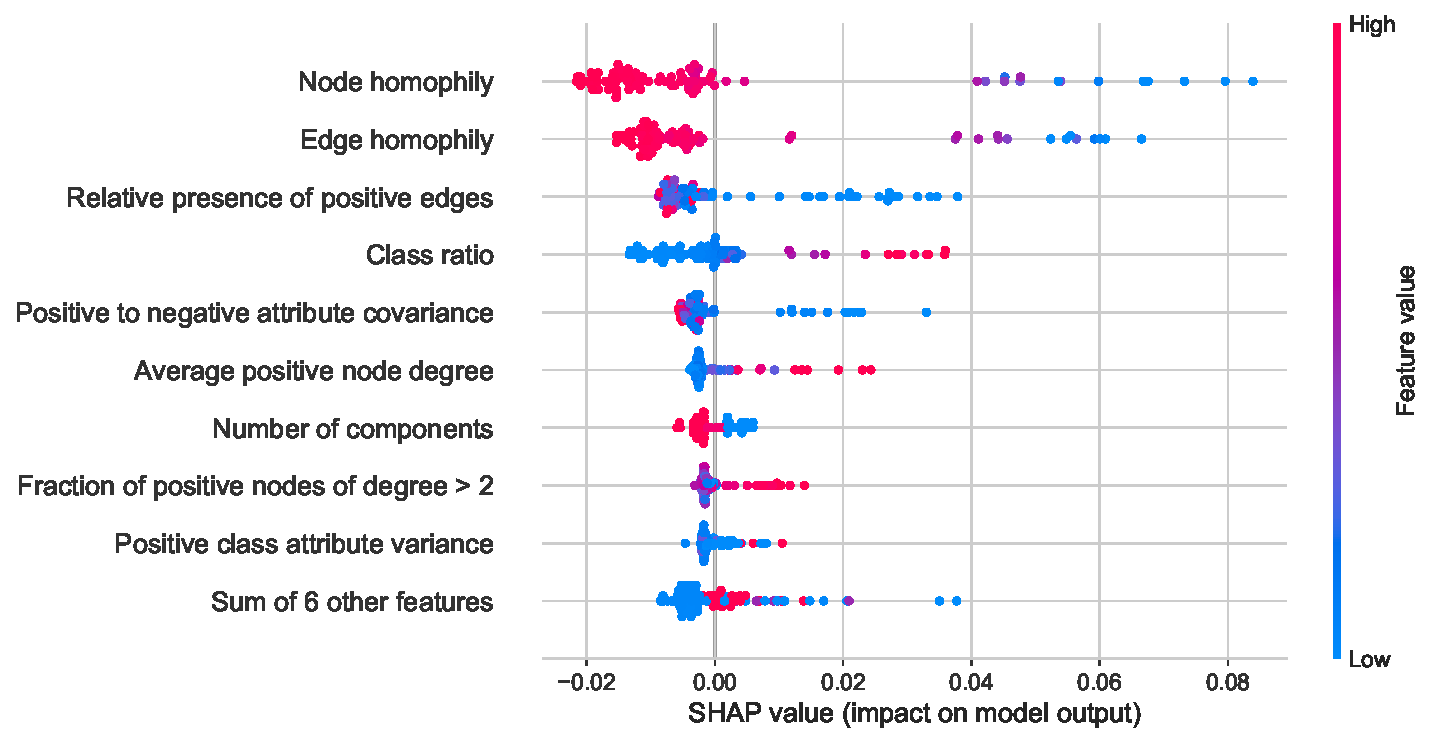
\includegraphics[width=\linewidth]{images/graph-property-importance.pdf}
\end{frame}

\section{Intended research directions}

\begin{frame}{Explainable graph models in cybersecurity}
	\begin{itemize}
		\item GNN models are black-boxes.
		\item Without clear explanations, security analysts might find it difficult to trust the model’s predictions, leading to skepticism or hesitation in acting upon the model’s recommendations
		\item By understanding why a model makes certain predictions, cybersecurity professionals can identify biases, correct inaccuracies, and refine algorithms to better detect evolving threats.
	\end{itemize}

	\vspace{10pt}
	{\Large Open questions}

	\begin{itemize}
		\item Which explanation algorithm is the most suitable for the domain?
		\item How to deal with hypergraphs?
		\item How to combine multiple modalities in one explanation?
		\item How to filter large graphs, while keeping the explanations relevant?
	\end{itemize}
\end{frame}

\begin{frame}{GNN hyper-parameter optimization guided by graph properties\footcite{prochazka_which_2023}}
	\begin{itemize}
		\item Expanding on the study of graph properties
		\item For each of the 139 datasets, we evaluated 108 hyper-parameter configurations.
		\item Meta-model predicting GraphSAGE performance
		\item Meta-model as hyper-parameter optimizer
	\end{itemize}

	\vfill

	\centering
	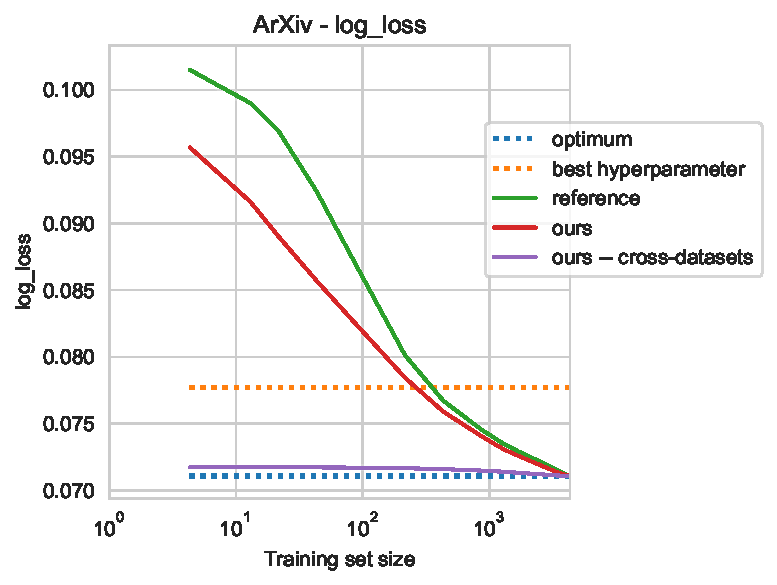
\includegraphics[width=0.6\linewidth]{images/hyperpar_tuning_single.pdf}
\end{frame}

\begin{frame}{Conclusion}
	\begin{itemize}
		\item Contributions
		\begin{itemize}
			\item Formalized the graph performance-complexity trade-off
			\item Introduced a HARP-based approach to solving it
			\item Introduced a simplified direct approach to solving it
			\item Studied the effect of graph properties on GNN performance
		\end{itemize}
		\item Intended research directions
		\begin{itemize}
			\item Applications in cybersecurity
			\item Explainable graph models
			\item Further exploration of the proposed hyper-parameter optimisation algorithm
		\end{itemize}
	\end{itemize}
\end{frame}

\begin{frame}
	\titlepage
\end{frame}

\section{Opponent's questions}

\begin{frame}{Opponent's questions}
	\textbf{Q1:} On figure 3.3, the performance of the downstream classifiers for ArXiv and Coauthors-CS graphs consistently improves, while other graphs achieve performance of the full model around 70\% mark, at the latest. Do you have any insights why the two graphs behave differently?
	\begin{center}
		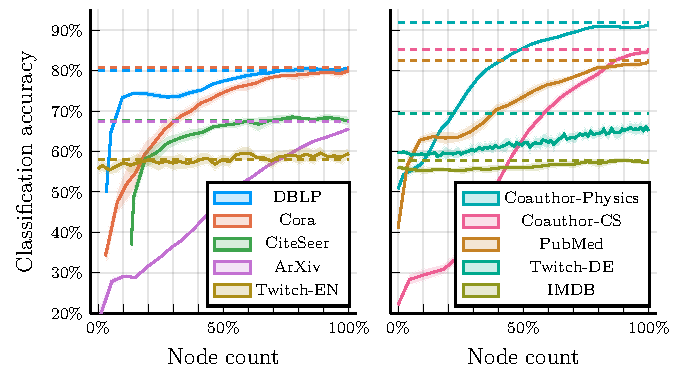
\includegraphics[width=0.5\pagewidth]{images/adaptive-coarsening/adaptive-coarsening.pdf}\footcite{dedic_balancing_2024}
	\end{center}

	\textbf{A:} We evaluated several graph metrics over the refinement procedure. The values of these metrics were compared to the classification accuracy and a strong correlation was found for the majority of them, with correlation coeffcient of −0.66 for global assortativity and between 0.94 and 0.96 for all the other metrics,.
\end{frame}

\begin{frame}{Opponent's questions}
	\textbf{Q2:} As for the coarsening of the graph, do you have a computational time analysis? How much time it takes to run the coarsening and what is the speedup of the ML model?

	\textbf{A:} We don't have a rigorous computational analysis. The coarsening algorithm generally scales linearly w.r.t.\ the number of nodes. On the experimental data, it took tenths of seconds to a few minutes to run, depending on the dataset. The graph algorithm itself also scales linearly w.r.t.\ the number of nodes.
\end{frame}

\begin{frame}{Opponent's questions}
	\textbf{Q3:} Have you considered a community detection algorithm (like Louvain algorithm) or some of its versions tailored to coarsening graphs for ML tasks?

	\textbf{A:} We haven't considered the Louvain algorithm specifically, but we have considered alternative coarsening schemes based on graph diffusion (Personalized PageRank \& Heat diffusion) and an evolved coarsening in our previous work \cite{dedic_adaptive_2022}.

	\centering
	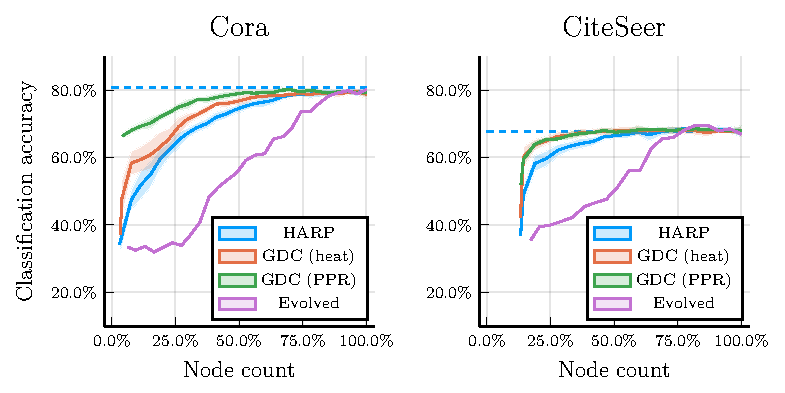
\includegraphics[width=0.7\pagewidth]{images/alternative-coarsening-algorithms/alternative-coarsening-algorithms.pdf}\footcite{dedic_adaptive_2022}
\end{frame}

\begin{frame}{Opponent's questions}
	\textbf{Q4:} It would be interesting to see how the generic coarsening algorithm (i.e.\ your CSP) compare to an informed (problem/data aware) heuristics and its effects on model’s performance and time-requirements.

	\textbf{A:} In \cite{prochazka_convolutional_2024}, we compared CSP with methods such as the Naive Bayes classifier, logistic regression, random forrests and hypergraph GCNs. Both performance and time requirements were compared.
\end{frame}

\begin{frame}{Opponent's questions}
	\textbf{Q5:} I would also look at meta-learning field and maybe there would be a way to steer the graph coarsening algorithms based on properties of a specific graph.

	\textbf{A:} A preliminary examination of that is covered in \cite{prochazka_scalable_2022}, but more research is needed. The interplay of meta-learning and graph properties is also the main topic of ongoing work outlined in Section 4.3, based on our previous work \cite{prochazka_which_2023}.
\end{frame}

\begin{frame}{Opponent's questions}
	\textbf{Q6:} What kind of cybersecurity do you have in mind? (Network monitoring, intrusion detection, malware detection, …) Do you have sources of cybersecurity related datasets? Do you have expert insights on the datasets?

	\textbf{A:} Network traffic analysis primarily. We do have in-house experts.
\end{frame}

\begin{frame}{Opponent's questions}
	\textbf{Q7:} How much work would be to transfer the approach to another domain (i.e.\ financial transaction analysis)?

	\textbf{A:} We haven't tried financial transaction analysis specifically, but include datasets from multiple domains:

	\begin{center}
		\adjustbox{width=\columnwidth}{%
			\begin{tabular}{lrrrrrrrrr}
				\toprule
				\textbf{Dataset} & \textbf{CiteSeer} & \textbf{Cora-CA}  & \textbf{Cora-CC}  & \textbf{DBLP} & \textbf{PubMed}   & \textbf{Corona} & \textbf{Walmar} & \textbf{movie-RA} & \textbf{movie-TA}\\
				\midrule
				\textbf{Node} & paper & paper & paper & paper & paper & text & product  & movie & movie \\
				\textbf{Node label} & topic & topic & topic & topic & topic & sentiment & category & category & category \\
				\textbf{Hyperedge} & citation & author & citation & author & citation & token & co-purchase & user & tag\\
				\midrule
				\textbf{Nodes}  & 3312 & 2708 & 2708 & 41302 & 19717 & 44955 & 88860 & 62423 & 62423\\
				\textbf{Isolated nodes} & 1854 & 320 & 1274 & 0 & 15877 & 0 & 1 & 3376 & 17172\\
				\textbf{Hyperedges}  & 1079 & 1072 & 1579 & 22363 & 7963 & 998 & 69906 & 162541 & 14592\\
				\( \boldsymbol{\Sigma}_E \)  & 3453 & 4585 & 4786 & 99561 & 34629 & 3455918 & 460629 & 25000095 & 1093360\\
				\textbf{Average \( \vdeg \left( v \right) \)} & 2.37 & 1.92 & 3.34 & 2.41 & 9.02 & 76.88 & 6.58 & 423.39 & 24.16\\
				\textbf{Average \( \edeg \left( e \right) \)} & 3.20 & 4.28 & 3.03 & 4.45 & 4.35 & 3463 & 5.18 & 153.8 & 74.9\\
				\textbf{Classes} & 6 & 7 & 7 & 6 & 3 & 5 & 11 & 20 & 20\\
				\bottomrule
			\end{tabular}
		}
	\end{center}
\end{frame}

\begin{frame}[allowframebreaks]{Bibliography}
	\printbibliography
\end{frame}

\end{document}
